\documentclass[aspectratio=169]{beamer}

% Shared Beamer settings for Applied Machine Learning lectures (UPES).
% Keep this file free of \documentclass to allow reuse via \input.

% Allow lecture sources to use shared theme/assets without copying them into each lecture folder.
% NOTE: These paths are relative to `Unit-xx/Lecture-yy/latex/` (and `Lab/Experiment-xx/latex/`).
\makeatletter
\def\input@path{{../../../_shared/}{../../../_shared/UPES-Beamer-Theme/}}
\makeatother

\usetheme{UPES}
\setbeamertemplate{navigation symbols}{}

\usepackage{amsmath}
\usepackage{amssymb}
\usepackage{booktabs}
\usepackage{graphicx}
\usepackage{hyperref}
\usepackage{xcolor}
\usepackage{listings}

% Code listings (Python-oriented for this subject).
\lstset{
  language=Python,
  basicstyle=\ttfamily\small,
  keywordstyle=\color{blue},
  commentstyle=\color{gray},
  stringstyle=\color{teal},
  showstringspaces=false,
  columns=fullflexible,
  breaklines=true
}

\usepackage{tikz}
\usetikzlibrary{arrows.meta,positioning,shapes.geometric,calc,fit,backgrounds}

% Per-slide source line (references shown on the slide itself).
\newcommand{\slidesources}[1]{%
  \vfill
  {\tiny\color{gray}\raggedright\sloppy\parbox{\linewidth}{Sources: #1}\par}%
}

% Unit-wise source strings for this subject (used by slides/notes).
% Path is relative to the lecture `latex/` folder (the compilation CWD).
% Source strings for Applied Machine Learning (CSAI2017P) — used by slides + notes.
% Prescribed texts and reference books are taken from the course syllabus.
% Support texts are the author-hosted open-access editions:
%   statlearning.com            (ISL with Python)
%   probml.github.io/pml-book   (Murphy, Probabilistic Machine Learning)
%   d2l.ai                      (Dive into Deep Learning)
%   mml-book.github.io          (Mathematics for Machine Learning)

\newcommand{\AMLRepoURL}{https://github.com/tali7c/Applied-Machine-Learning}

% --- prescribed -------------------------------------------------------------
\newcommand{\AMLPrescribed}{%
M\"uller and Guido, \textit{Introduction to Machine Learning with Python}, O'Reilly, 2016.;%
Bishop, \textit{Pattern Recognition and Machine Learning}, Springer, 2006.;%
Murphy, \textit{Machine Learning: A Probabilistic Perspective}, MIT Press, 2012.;%
Han, Kamber and Pei, \textit{Data Mining: Concepts and Techniques} (3e), Morgan Kaufmann, 2012.%
}

% --- unit-wise ---------------------------------------------------------------
\newcommand{\AMLUnitISources}{%
M\"uller and Guido, \textit{Introduction to Machine Learning with Python}, Ch. 1.;%
Bishop, \textit{Pattern Recognition and Machine Learning}, Ch. 1.;%
Murphy, \textit{Probabilistic Machine Learning: An Introduction}, MIT Press, 2022, Ch. 1.;%
Mitchell, \textit{Machine Learning}, McGraw Hill, 1997, Ch. 1.;%
Scikit-learn documentation, accessed 2026-08-04.%
}

\newcommand{\AMLUnitIISources}{%
Bishop, \textit{Pattern Recognition and Machine Learning}, \S1.5, \S4.3, \S7.1.;%
Zhang, Lipton, Li and Smola, \textit{Dive into Deep Learning}, \S3.4.;%
Shalev-Shwartz and Ben-David, \textit{Understanding Machine Learning}, Ch. 15.;%
Murphy, \textit{Probabilistic Machine Learning: An Introduction}, Ch. 5.%
}

\newcommand{\AMLUnitIIISources}{%
Zhang, Lipton, Li and Smola, \textit{Dive into Deep Learning}, Ch. 12 (Optimization Algorithms).;%
Deisenroth, Faisal and Ong, \textit{Mathematics for Machine Learning}, Ch. 7.;%
Kingma and Ba, ``Adam: A Method for Stochastic Optimization,'' ICLR 2015.;%
Ruder, ``An overview of gradient descent optimization algorithms,'' arXiv:1609.04747, 2016.%
}

\newcommand{\AMLUnitIVSources}{%
Han, Kamber and Pei, \textit{Data Mining: Concepts and Techniques} (3e), Ch. 3.;%
M\"uller and Guido, \textit{Introduction to Machine Learning with Python}, Ch. 3--4.;%
James, Witten, Hastie, Tibshirani and Taylor, \textit{An Introduction to Statistical Learning with Python}, Ch. 5--6, 12.;%
Scikit-learn documentation (preprocessing, model selection), accessed 2026-08-04.%
}

\newcommand{\AMLUnitVSources}{%
James et al., \textit{An Introduction to Statistical Learning with Python}, Ch. 3--6.;%
Bishop, \textit{Pattern Recognition and Machine Learning}, Ch. 3.;%
Deisenroth, Faisal and Ong, \textit{Mathematics for Machine Learning}, Ch. 9.;%
M\"uller and Guido, \textit{Introduction to Machine Learning with Python}, \S2.3.%
}

\newcommand{\AMLUnitVISources}{%
Han, Kamber and Pei, \textit{Data Mining: Concepts and Techniques} (3e), Ch. 8--9.;%
James et al., \textit{An Introduction to Statistical Learning with Python}, Ch. 8--9.;%
Bishop, \textit{Pattern Recognition and Machine Learning}, Ch. 4--5, 7, 14.;%
Zhang et al., \textit{Dive into Deep Learning}, Ch. 5.%
}

\newcommand{\AMLUnitVIISources}{%
Han, Kamber and Pei, \textit{Data Mining: Concepts and Techniques} (3e), Ch. 10.;%
James et al., \textit{An Introduction to Statistical Learning with Python}, Ch. 12.;%
M\"uller and Guido, \textit{Introduction to Machine Learning with Python}, \S3.5.;%
Ester, Kriegel, Sander and Xu, ``A density-based algorithm for discovering clusters (DBSCAN),'' KDD 1996.%
}

\newcommand{\AMLLabSources}{%
M\"uller and Guido, \textit{Introduction to Machine Learning with Python}, companion notebooks.;%
McKinney, \textit{Python for Data Analysis} (3e), O'Reilly, 2022.;%
Scikit-learn user guide, accessed 2026-08-04.;%
Matplotlib and Seaborn documentation, accessed 2026-08-04.%
}



\graphicspath{{../figures/}{../images/}{../../../_shared/}{../../../_shared/UPES-Beamer-Theme/}}

\title[Applied Machine Learning]{Applied Machine Learning}
\subtitle{Unit 06 -- Lecture 18: Support Vector Machines}
\author{Tofik Ali}
\institute{School of Computer Science, UPES Dehradun}
\date{Autumn 2026}

% ---- a compact "output" block so code and its result sit together ----------
\lstdefinestyle{outblk}{
  basicstyle=\ttfamily\scriptsize\color{black!75},
  backgroundcolor=\color{black!5}, frame=leftline, framerule=2pt,
  rulecolor=\color{black!30}, breaklines=true, columns=fullflexible,
  keepspaces=true,   % several outputs below are aligned tables
  language={},       % printed output is not Python: do not syntax-highlight it
  xleftmargin=4pt, aboveskip=1pt, belowskip=1pt, literate={-}{{-}}1}
\lstnewenvironment{outblk}{\lstset{style=outblk}}{}

\begin{document}

\UPESCoverFrame
\setcounter{framenumber}{0}

\begin{frame}
  \titlepage
  \begin{center}
    \footnotesize Of all the lines that separate the data, one is furthest
    from it\\[0.25em]
    \footnotesize Topic focus: \textbf{the margin, and the handful of points
    that set it}\\[0.25em]
    \footnotesize Repository: \texttt{\AMLRepoURL}
  \end{center}
  \slidesources{\AMLUnitVISources}
\end{frame}

\begin{frame}{Quick Links}
  \centering
  \hyperlink{sec:margin}{\beamerbutton{The maximum margin}}\hspace{0.4em}
  \hyperlink{sec:dual}{\beamerbutton{Primal, Lagrangian, dual}}\hspace{0.4em}
  \hyperlink{sec:sv}{\beamerbutton{Support vectors}}\hspace{0.4em}
  \hyperlink{sec:soft}{\beamerbutton{Soft margin and $C$}}\\[0.6em]
  \hyperlink{sec:hinge}{\beamerbutton{The hinge loss}}\hspace{0.4em}
  \hyperlink{sec:kernel}{\beamerbutton{The kernel trick}}\hspace{0.4em}
  \hyperlink{sec:practice}{\beamerbutton{$\gamma$, scaling, cost}}\hspace{0.4em}
  \hyperlink{sec:summary}{\beamerbutton{Summary}}
\end{frame}

\begin{frame}{Agenda}
  \tableofcontents
\end{frame}

\begin{frame}[shrink=8]{How this lecture works}
  \begin{columns}[T]
    \begin{column}{0.48\textwidth}
      \begin{block}{Every idea appears twice}
        \begin{enumerate}
          \item \textbf{By hand} --- six points on graph paper, two vectors
            with small integer entries, one multiplier per support vector.
            Small enough that every number can be checked with a pen.
          \item \textbf{In code} --- the same arithmetic, then the same
            arithmetic again inside \texttt{scikit-learn}, so you can see
            that \texttt{SVC} returns \emph{exactly} the coefficients you
            worked out and nothing magic.
        \end{enumerate}
      \end{block}
    \end{column}
    \begin{column}{0.48\textwidth}
      \begin{alertblock}{Commit before you look}
        Four slides ask you to predict a number before it is revealed. Write
        your guess down. Being wrong on paper is how the idea sticks.
      \end{alertblock}
    \end{column}
  \end{columns}
  \vspace{0.3em}
  \begin{center}
    \small The centrepiece is \textbf{six points solved completely by hand}:
    $w = (1,1)$, $b = -3$, two support vectors, margin width $\sqrt2$, and
    both multipliers equal to $1$. Then we delete one point at a time and
    watch what does and does not move.
  \end{center}
\end{frame}

\begin{frame}[shrink=5]{Where we are}
  \begin{columns}[T]
    \begin{column}{0.47\textwidth}
      \begin{block}{Two lectures ago the objection was instability}
        A single tree moves when you move a few rows. Ensembles answered that
        by averaging many unstable models.
      \end{block}
      \begin{block}{This lecture answers it a different way}
        Build \emph{one} boundary, and choose the one that is as far as
        possible from every training point. A boundary with room around it
        does not move when the data jiggles --- because most of the data was
        never touching it.
      \end{block}
    \end{column}
    \begin{column}{0.49\textwidth}
      \begin{exampleblock}{Today's one question}
        A hundred different lines separate these two classes perfectly.
        \emph{Which one should I pick?}
      \end{exampleblock}
      \begin{alertblock}{And a promise for the second half}
        We will take a dataset that \textbf{no line can separate}, and
        classify it perfectly with a linear model --- without ever computing
        the coordinates of the space in which it becomes linear. That is the
        kernel trick, and we will verify the identity that makes it work
        rather than assert it.
      \end{alertblock}
    \end{column}
  \end{columns}
\end{frame}

\begin{frame}[shrink=6]{One seed --- and the one thing no seed can fix}
  \begin{columns}[T]
    \begin{column}{0.48\textwidth}
      \begin{block}{The one seed}
        \small Everything arbitrary in this deck uses \textbf{seed $0$}:
        the cross-validation shuffle
        (\texttt{StratifiedKFold(5, shuffle=True, random\_state=0)}), the
        train/test split, the solver permutations. Every listing shows it.
      \end{block}
      \begin{exampleblock}{A fit with no seed at all}
        \small Given its data, an \texttt{SVC} fit is \emph{deterministic}.
        Every accuracy, every support-vector count, every dual coefficient in
        this deck reproduces exactly.
      \end{exampleblock}
    \end{column}
    \begin{column}{0.48\textwidth}
      \begin{block}{Seeds that define data}
        \small \texttt{make\_blobs(random\_state=3)},
        \texttt{make\_moons(random\_state=3)},
        \texttt{make\_circles(random\_state=0)},
        \texttt{make\_classification(random\_state=0)}. These do not
        randomise an experiment --- they \emph{are} the dataset. They never
        move.
      \end{block}
      \begin{alertblock}{And the exception}
        \small The cost section reports \textbf{seconds}. No seed fixes a
        clock. Quote the support-vector counts beside them instead.
      \end{alertblock}
    \end{column}
  \end{columns}
\end{frame}

% =====================================================================
\section[Maximum margin]{The maximum-margin idea}
\label{sec:margin}

\begin{frame}[shrink=6]{Six points, and more separating lines than you can draw}
  \begin{columns}[T]
    \begin{column}{0.46\textwidth}
      \begin{block}{The data}
        \small
        \begin{tabular}{clr}
          \toprule
          point & $x$ & $y$ \\
          \midrule
          A & $(1,1)$ & $-1$ \\
          B & $(0,1)$ & $-1$ \\
          C & $(1,0)$ & $-1$ \\
          D & $(2,2)$ & $+1$ \\
          E & $(3,2)$ & $+1$ \\
          F & $(2,3)$ & $+1$ \\
          \bottomrule
        \end{tabular}
      \end{block}
      \begin{exampleblock}{}
        \small Every line in the picture gets all six right. Training
        accuracy cannot tell them apart.
      \end{exampleblock}
    \end{column}
    \begin{column}{0.52\textwidth}
      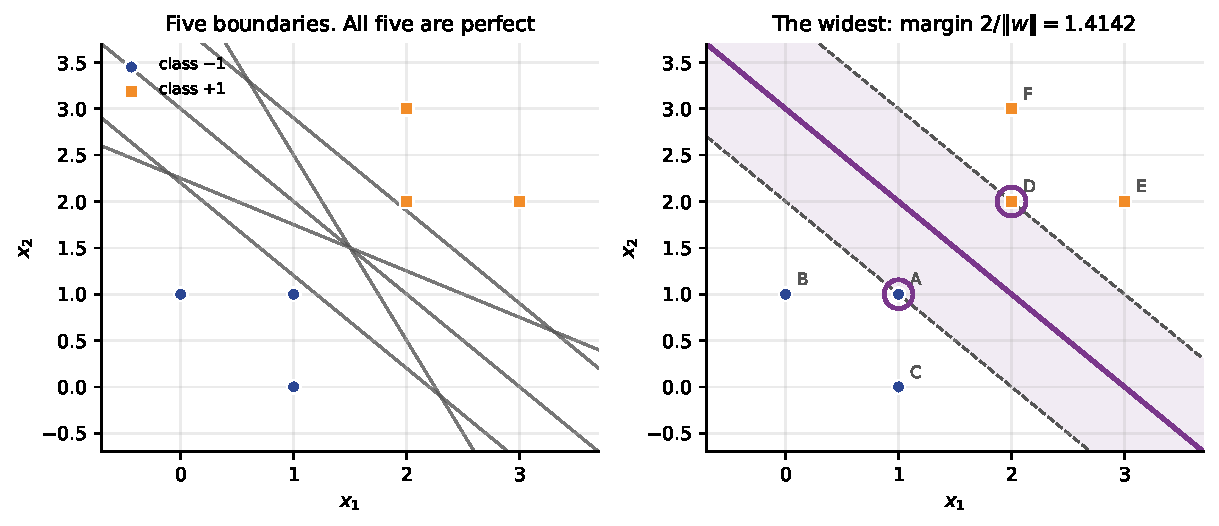
\includegraphics[width=\textwidth]{manylines.pdf}
    \end{column}
  \end{columns}
\end{frame}

\begin{frame}{Predict first \#1 --- which line would you bet on?}
  \begin{alertblock}{Commit to an answer}
    Five candidate lines, all with zero training errors. Rank them by how
    \emph{safe} they look, and then put a number on it: for the line
    $x_1 + x_2 - 3 = 0$, how far is the nearest of the six points?

    \medskip
    \centering\large
    Distance $=$ ? \qquad and how does it compare with $x_1+x_2-3.9=0$?
  \end{alertblock}
  \onslide<2->{
  \begin{exampleblock}{}
    \centering
    $x_1+x_2-3=0$ has its nearest point at $\mathbf{0.7071}$;
    $x_1+x_2-3.9=0$ at $\mathbf{0.0707}$ --- ten times closer, same accuracy.
  \end{exampleblock}}
\end{frame}

\begin{frame}[fragile]{The same five lines, measured}
\begin{outblk}
  line                    errors   nearest point   margin width
  1x1 +1x2 -2.2 = 0            0          0.1414         0.2828
  1x1 +1x2 -3.9 = 0            0          0.0707         0.1414
  2x1 +1x2 -4.5 = 0            0          0.6708         1.3416
  1x1 +2x2 -4.5 = 0            0          0.6708         1.3416
  1x1 +1x2 -3 = 0              0          0.7071         1.4142
every one of them is a perfect classifier; they are not equally safe
\end{outblk}
  \begin{center}\small
    \textbf{Accuracy is blind to this entirely.} The last line has ten times
    the clearance of the second and scores identically on the training set.
    The whole of today is a way of making that difference into an objective a
    solver can optimise.
  \end{center}
\end{frame}

\begin{frame}[shrink=4]{Distance from a point to a hyperplane}
  A hyperplane is $\{x : w^\top x + b = 0\}$. The vector $w$ is perpendicular
  to it: if $x$ and $x'$ both lie on it, $w^\top(x - x') = 0$.
  \begin{columns}[T]
    \begin{column}{0.52\textwidth}
      \begin{block}{The signed distance}
        Write $x = x_p + r\,\frac{w}{\|w\|}$, with $x_p$ the foot of the
        perpendicular. Then
        \[
          w^\top x + b
          = \underbrace{w^\top x_p + b}_{=\,0} + r\,\frac{w^\top w}{\|w\|}
          = r\,\|w\|,
        \]
        so the distance is
        $\displaystyle r = \frac{w^\top x + b}{\|w\|}.$
      \end{block}
    \end{column}
    \begin{column}{0.44\textwidth}
      \begin{alertblock}{Two different margins}
        \textbf{Functional} margin: $\hat\gamma_i = y_i(w^\top x_i + b)$.\\[0.3em]
        \textbf{Geometric} margin:
        $\gamma_i = \hat\gamma_i / \|w\|$.\\[0.4em]
        Doubling $w$ and $b$ doubles the functional margin and leaves the
        geometric one alone --- and leaves the boundary exactly where it was.
      \end{alertblock}
    \end{column}
  \end{columns}
\end{frame}

\begin{frame}[shrink=6]{Deriving the width: the margin is $2/\|w\|$}
  \begin{block}{Kill the redundancy first}
    $(w,b)$ and $(cw,cb)$ describe the \emph{same} boundary for any $c>0$.
    Fix the scale by demanding that the closest points have functional
    margin exactly one:
    \[
      \min_i\, y_i\,(w^\top x_i + b) = 1.
      \qquad\text{(the \emph{canonical} hyperplane)}
    \]
  \end{block}
  \begin{columns}[T]
    \begin{column}{0.52\textwidth}
      \begin{exampleblock}{The consequence}
        A closest point of class $+1$ satisfies $w^\top x + b = +1$; one of
        class $-1$ satisfies $w^\top x + b = -1$. Their distances from the
        boundary are $1/\|w\|$ each, so the empty band between them has width
        \[
          \boxed{\ \frac{2}{\|w\|}\ }
        \]
      \end{exampleblock}
    \end{column}
    \begin{column}{0.44\textwidth}
      \begin{alertblock}{And therefore}
        \[
          \max \frac{2}{\|w\|}
          \iff \min \|w\|
          \iff \min \tfrac12\|w\|^2 .
        \]
        The $\tfrac12$ and the square are there only to make the derivative
        tidy; they change nothing about where the minimum is.
      \end{alertblock}
    \end{column}
  \end{columns}
\end{frame}

\begin{frame}[shrink=12]{The whole problem, in one box --- and drawn}
  \begin{exampleblock}{The hard-margin primal}
    \[
      \min_{w,\,b}\ \tfrac12 \|w\|^2
      \qquad\text{subject to}\qquad
      y_i\,(w^\top x_i + b) \ \ge\ 1
      \quad\text{for } i = 1,\dots,n .
    \]
  \end{exampleblock}
  \begin{center}
    
\includegraphics[width=0.56\textwidth]{margin.pdf}
  \end{center}
  \begin{center}\small
    $w = (1,1)$, $b = -3$, $\|w\| = \sqrt2$, so the band is
    $2/\|w\| = \mathbf{1.414214}$ wide; \textbf{A} and \textbf{D} sit exactly
    on its edges. The constraint says two things at once --- correct side
    \emph{and} at least one functional unit clear. This is a
    \textbf{convex quadratic program}: one global optimum, no local minima to
    get stuck in. And note what is \emph{absent} from the objective --- any
    count of how many points are correct.
  \end{center}
\end{frame}

% =====================================================================
\section[Primal and dual]{The primal, the Lagrangian and the dual}
\label{sec:dual}

\begin{frame}[shrink=4]{Attaching a multiplier to every constraint}
  \begin{block}{The Lagrangian}
    Introduce one multiplier $\alpha_i \ge 0$ per training point:
    \[
      L(w,b,\alpha) \;=\; \tfrac12\|w\|^2
        \;-\; \sum_{i=1}^{n} \alpha_i\bigl[\,y_i(w^\top x_i + b) - 1\,\bigr].
    \]
  \end{block}
  \begin{columns}[T]
    \begin{column}{0.48\textwidth}
      \begin{exampleblock}{Stationarity}
        \[
          \frac{\partial L}{\partial w} = 0
          \;\Longrightarrow\;
          w = \sum_i \alpha_i y_i x_i
        \]
        \[
          \frac{\partial L}{\partial b} = 0
          \;\Longrightarrow\;
          \sum_i \alpha_i y_i = 0
        \]
      \end{exampleblock}
    \end{column}
    \begin{column}{0.48\textwidth}
      \begin{alertblock}{Read the first one again}
        $w$ is a \textbf{weighted sum of the training points themselves}. The
        model does not invent a direction; it combines the data. Any point
        with $\alpha_i = 0$ contributes nothing to that sum.
      \end{alertblock}
    \end{column}
  \end{columns}
\end{frame}

\begin{frame}[shrink=6]{Substituting back gives the dual}
  Put $w = \sum_i \alpha_i y_i x_i$ and $\sum_i \alpha_i y_i = 0$ back into
  $L$. The $b$ term vanishes, the cross terms collapse, and what is left
  contains the data \emph{only} through inner products:
  \begin{exampleblock}{The dual problem}
    \[
      \max_{\alpha}\ \sum_{i=1}^{n}\alpha_i
        - \tfrac12 \sum_{i=1}^{n}\sum_{j=1}^{n}
          \alpha_i\alpha_j\,y_i y_j\, \langle x_i, x_j\rangle
      \quad\text{s.t.}\quad
      \alpha_i \ge 0,\ \ \sum_i \alpha_i y_i = 0 .
    \]
  \end{exampleblock}
  \begin{columns}[T]
    \begin{column}{0.48\textwidth}
      \begin{block}{Why anyone bothers}
        The problem is now in $n$ variables instead of $d+1$, which is a win
        when $d \gg n$ --- and, far more importantly, $x$ appears
        \textbf{only} inside $\langle x_i, x_j\rangle$.
      \end{block}
    \end{column}
    \begin{column}{0.48\textwidth}
      \begin{alertblock}{Hold on to that}
        Everything in the kernel section follows from this one
        observation. If the algorithm only ever needs inner products, you can
        change what ``inner product'' means without changing the algorithm.
      \end{alertblock}
    \end{column}
  \end{columns}
\end{frame}

\begin{frame}[shrink=5]{The KKT conditions, and the sentence that matters}
  \begin{block}{At the optimum of a convex problem with linear constraints}
    \[
      \alpha_i \ge 0, \qquad
      y_i(w^\top x_i + b) - 1 \ge 0, \qquad
      \underbrace{\alpha_i\bigl[\,y_i(w^\top x_i + b) - 1\,\bigr] = 0}
        _{\textbf{complementary slackness}} .
    \]
  \end{block}
  \begin{columns}[T]
    \begin{column}{0.48\textwidth}
      \begin{exampleblock}{A product of two things is zero}
        So for every single point, \emph{at least one factor is zero}:
        \begin{itemize}
          \item either $\alpha_i = 0$ --- the point is irrelevant;
          \item or $y_i(w^\top x_i + b) = 1$ --- the point sits exactly on
            the margin.
        \end{itemize}
      \end{exampleblock}
    \end{column}
    \begin{column}{0.48\textwidth}
      \begin{alertblock}{The definition, earned rather than announced}
        \centering\large
        The points with $\alpha_i > 0$ are the\\ \textbf{support vectors}.

        \smallskip
        \normalsize Everything else could be deleted and the answer would not
        change. We are about to do exactly that.
      \end{alertblock}
    \end{column}
  \end{columns}
\end{frame}

\begin{frame}[shrink=6]{By hand: solving the six points completely}
  \begin{columns}[T]
    \begin{column}{0.50\textwidth}
      \begin{block}{Guess the support set, then verify}
        The two closest points across the classes are A$(1,1)$ and D$(2,2)$.
        Suppose only those two have $\alpha > 0$. Then
        $\sum_i\alpha_i y_i = 0$ gives
        $-\alpha_A + \alpha_D = 0$, so $\alpha_A = \alpha_D = \alpha$, and
        \[
          w = \alpha\bigl[(2,2)-(1,1)\bigr] = \alpha\,(1,1).
        \]
      \end{block}
    \end{column}
    \begin{column}{0.46\textwidth}
      \begin{exampleblock}{Two equations, two unknowns}
        Both are on the margin, so
        \[
          -\bigl(2\alpha + b\bigr) = 1,
          \qquad
          4\alpha + b = 1 .
        \]
        Add them: $2\alpha = 2$, so $\boxed{\alpha = 1}$ and
        $b = 1 - 4 = \boxed{-3}$, giving $w = \boxed{(1,1)}$.
      \end{exampleblock}
    \end{column}
  \end{columns}
  \vspace{0.2em}
  \begin{center}\small
    Check the other four: B and C give $w^\top x + b = -2$, so
    $y_i f = 2 > 1$; E and F give $+2$, so $y_i f = 2 > 1$. Every constraint
    holds, so the guess was right. Width $2/\|w\| = 2/\sqrt2 = 1.414214$.
  \end{center}
\end{frame}

\begin{frame}[fragile,shrink=4]{The same thing in code --- to ten decimal places}
\begin{lstlisting}
X = np.array([[1.,1.],[0.,1.],[1.,0.],[2.,2.],[3.,2.],[2.,3.]])
y = np.array([-1,-1,-1, 1, 1, 1])
clf = SVC(kernel="linear", C=1e6).fit(X, y)   # C huge = hard margin
\end{lstlisting}
\begin{outblk}
by hand :  w = (1, 1)   b = -3
           ||w||   = 1.4142135624
           2/||w|| = 1.4142135624
SVC     :  w = [1. 1.]   b = -3.0000000000
           2/||w|| = 1.4142135624
agree to 1e-9: True
\end{outblk}
  \begin{center}\small
    Not ``close to''. \textbf{The same numbers.} The library solved the same
    quadratic program you just solved with two linear equations.
  \end{center}
\end{frame}

\begin{frame}[fragile,shrink=6]{The multipliers, and $w$ rebuilt from them}
\begin{lstlisting}
alpha = np.zeros(len(X)); alpha[clf.support_] = np.abs(clf.dual_coef_[0])
w_dual = (alpha * y) @ X
\end{lstlisting}
\begin{outblk}
support_        : [0 3] -> A D
alpha           : [1. 0. 0. 1. 0. 0.]
sum_i alpha_i y_i = 0.0e+00   (must be 0)
w = sum_i alpha_i y_i x_i = [1. 1.]
b = mean over SVs of (y_s - w.x_s) = -3.0000000000
dual objective  = 1.0000000000
(1/2)||w||^2    = 1.0000000000
\end{outblk}
  \begin{center}\small
    Four of the six multipliers are \textbf{exactly zero}. The dual objective
    equals the primal objective, which is what \emph{strong duality} means:
    solving either one solves the other.
  \end{center}
\end{frame}

\begin{frame}[fragile,shrink=10]{Which points are on the margin? Read $y_i f(x_i)$}
  \begin{columns}[T]
    \begin{column}{0.46\textwidth}
\begin{outblk}
pt   f(x)     y f(x)   on the margin?
 A   -1.00    +1.00       yes
 B   -2.00    +2.00       no
 C   -2.00    +2.00       no
 D   +1.00    +1.00       yes
 E   +2.00    +2.00       no
 F   +2.00    +2.00       no
\end{outblk}
      \begin{center}\small
        $y_i f(x_i) = 1$ exactly on the margin, $>1$ strictly outside.
        Compare against the $\alpha$ column: complementary slackness,
        printed twice.
      \end{center}
    \end{column}
    \begin{column}{0.52\textwidth}
      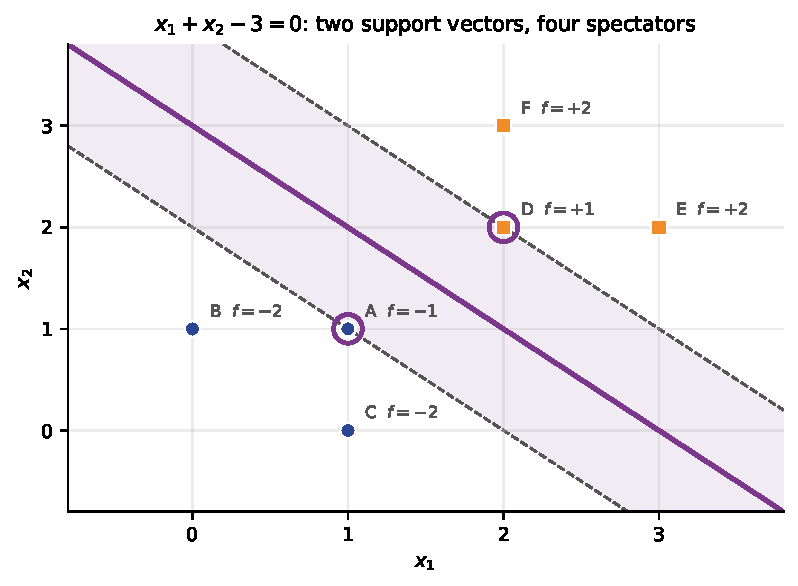
\includegraphics[width=\textwidth]{handsvm.pdf}
      \begin{center}\small
        Two rings, two non-zero multipliers, both equal to $1$. One line,
        fixed by two points --- the smallest number that can fix a line in
        the plane, one from each side.
      \end{center}
    \end{column}
  \end{columns}
\end{frame}

% =====================================================================
\section[Support vectors]{Support vectors: the memorable result}
\label{sec:sv}

\begin{frame}{Predict first \#2 --- delete a point}
  \begin{alertblock}{Commit to two answers}
    I am going to refit the SVM twice on five points instead of six.
    \begin{enumerate}
      \item First I delete \textbf{B} at $(0,1)$, which is not a support
        vector. What happens to $w$, to $b$ and to the margin width?
      \item Then I put B back and delete \textbf{A} at $(1,1)$, which is.
        Same three questions.
    \end{enumerate}
    \medskip
    \centering\large
    Write down both answers before the next slide.
  \end{alertblock}
  \onslide<2->{
  \begin{center}\small
    Almost everyone gets the first one right in words (``nothing happens'')
    and hedges. It is worth being precise: \emph{nothing happens} means the
    difference is $0.00\mathrm{e}{+00}$, not ``a small change''.
  \end{center}}
\end{frame}

\begin{frame}[fragile,shrink=8]{The reveal --- one deletion is free, the other is not}
\begin{outblk}
all six points             w = (1.0000, 1.0000)  b = -3.0000  nSV = 2  2/||w|| = 1.4142
drop B (0,1), not a SV     w = (1.0000, 1.0000)  b = -3.0000  nSV = 2  2/||w|| = 1.4142
drop D (2,2), a SV         w = (0.6665, 0.6670)  b = -2.3337  nSV = 3  2/||w|| = 2.1211
drop A (1,1), a SV         w = (0.6664, 0.6668)  b = -1.6665  nSV = 3  2/||w|| = 2.1215
dropping B moved w by 0.00e+00 and b by 0.00e+00 -- nothing moved
dropping a support vector widened the margin 1.4142 -> 2.1211
\end{outblk}
  \begin{center}
    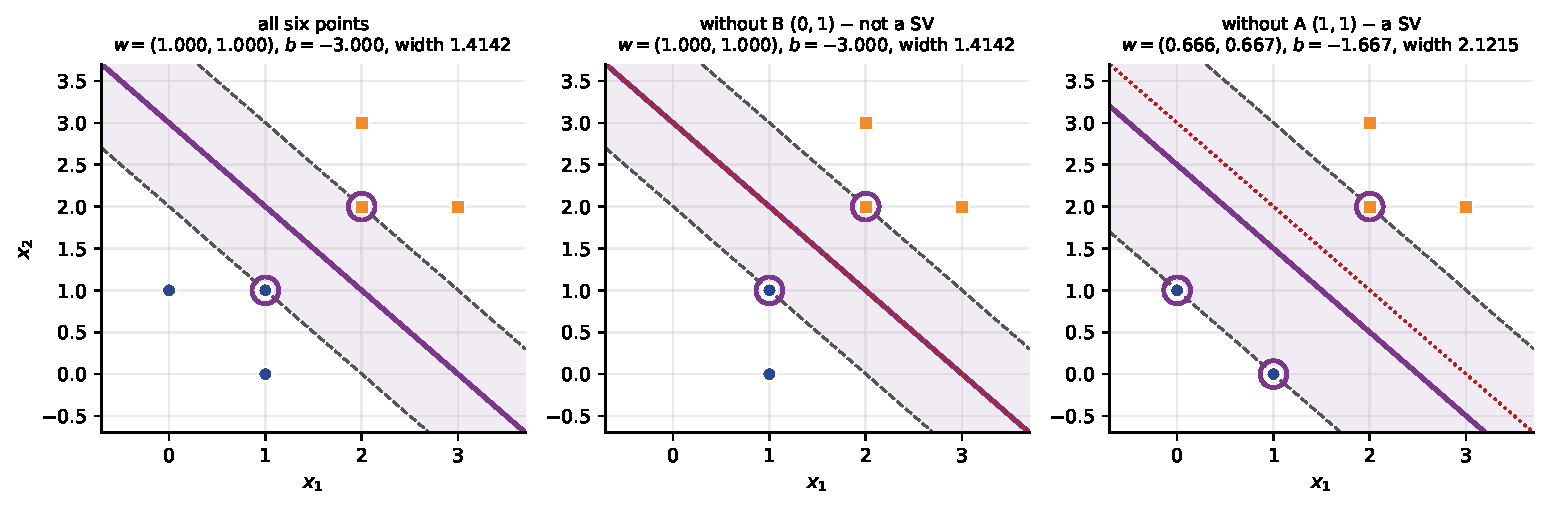
\includegraphics[width=0.86\textwidth]{deletion.pdf}
  \end{center}
\end{frame}

\begin{frame}[shrink=6]{Why the margin got \emph{wider}}
  \begin{columns}[T]
    \begin{column}{0.50\textwidth}
      \begin{block}{Constraints only ever hurt}
        Deleting a point removes a constraint from the primal. A minimisation
        over a \emph{larger} feasible set can only do the same or better, so
        $\tfrac12\|w\|^2$ can only fall --- and a smaller $\|w\|$ is a wider
        band.
      \end{block}
      \begin{exampleblock}{Check it by hand}
        Without A, the nearest negative to the positives is the midpoint of
        B$(0,1)$ and C$(1,0)$, at $(0.5,0.5)$; the nearest positive is
        D$(2,2)$. The gap is $\|(1.5,1.5)\| = 2.1213$, and
        $2/\|w\| = 2.1215$. Agreement to four decimal places.
      \end{exampleblock}
    \end{column}
    \begin{column}{0.46\textwidth}
      \begin{alertblock}{The examinable sentence}
        \centering
        \textbf{The support vectors are the training set.}\\[0.4em]
        \normalsize Delete every other row and you get the identical model.
        Delete one support vector and the boundary moves. That is what
        $\alpha_i = 0$ \emph{means}.
      \end{alertblock}
      \begin{block}{And a warning}
        The same property makes an SVM sensitive to an outlier that happens
        to sit near the boundary --- it becomes a support vector and drags
        the whole model. The soft margin exists to blunt this.
      \end{block}
    \end{column}
  \end{columns}
\end{frame}

\begin{frame}[fragile,shrink=4]{Not a toy effect: throw away $69$ of $80$ rows}
\begin{lstlisting}
full = SVC(kernel="linear", C=1.0).fit(Xb, yb)          # 80 points
only = SVC(kernel="linear", C=1.0).fit(Xb[full.support_], yb[full.support_])
\end{lstlisting}
\begin{outblk}
trained on all 80 points : w = [-0.976353 -0.408819]  b = -1.475724
trained on the 11 SVs only: w = [-0.975901 -0.40859 ]  b = -1.475336
identical predictions on all 80 points: True
the other 69 rows changed nothing
\end{outblk}
  \begin{center}\small
    $86\%$ of the training set could be deleted after the fact with no change
    to a single prediction. The coefficients differ in the fourth decimal
    only because the solver stops at its tolerance, not because the answer is
    different.
  \end{center}
\end{frame}

% =====================================================================
\section[Soft margin]{The soft margin and $C$}
\label{sec:soft}

\begin{frame}[shrink=5]{Real data is not separable, and hard margin then fails}
  \begin{columns}[T]
    \begin{column}{0.48\textwidth}
      \begin{alertblock}{The hard-margin problem is infeasible}
        If no hyperplane separates the classes, there is no $(w,b)$
        satisfying every $y_i(w^\top x_i + b)\ge 1$. The feasible set is
        empty. The solver does not return a poor answer; there is no answer.
      \end{alertblock}
    \end{column}
    \begin{column}{0.48\textwidth}
      \begin{block}{Buy your way out with slack}
        Give each point a \textbf{slack variable} $\xi_i \ge 0$ and let it
        fall short:
        \[
          y_i(w^\top x_i + b) \ \ge\ 1 - \xi_i .
        \]
        Then charge for it in the objective.
      \end{block}
    \end{column}
  \end{columns}
  \vspace{0.2em}
  \begin{exampleblock}{The soft-margin primal}
    \[
      \min_{w,b,\xi}\ \ \tfrac12\|w\|^2 \;+\; C\sum_{i=1}^{n}\xi_i
      \qquad\text{s.t.}\qquad
      y_i(w^\top x_i + b) \ge 1 - \xi_i,\quad \xi_i \ge 0 .
    \]
  \end{exampleblock}
\end{frame}

\begin{frame}[shrink=6]{What $\xi_i$ measures, in three cases}
  \begin{columns}[T]
    \begin{column}{0.33\textwidth}
      \begin{block}{$\xi_i = 0$}
        The point is outside the margin, on the right side. It has paid
        nothing. Most points are here.
      \end{block}
    \end{column}
    \begin{column}{0.33\textwidth}
      \begin{block}{$0 < \xi_i \le 1$}
        Inside the margin band but still correctly classified. It costs
        something even though the prediction is right.
      \end{block}
    \end{column}
    \begin{column}{0.33\textwidth}
      \begin{block}{$\xi_i > 1$}
        Past the boundary --- \textbf{misclassified}. The count of these is
        the training error.
      \end{block}
    \end{column}
  \end{columns}
  \vspace{0.3em}
  \begin{exampleblock}{}
    \centering
    $\xi_i = \max\bigl(0,\ 1 - y_i f(x_i)\bigr)$ --- and you have met that
    function before. Hold that thought for two slides.
  \end{exampleblock}
  \begin{center}\small
    The dual is \emph{unchanged} except that $\alpha_i \ge 0$ becomes
    $0 \le \alpha_i \le C$. That single box constraint is the entire
    mathematical content of the soft margin.
  \end{center}
\end{frame}

\begin{frame}[fragile,shrink=6]{$C$ trades margin width against violations}
\begin{outblk}
     C   nSV   2/||w||   sum of slacks   inside margin   wrong side   train acc
  0.01    35    5.2135         17.8304               32            3      0.9625
   0.1    18    2.1750          8.3313               15            3      0.9625
     1    11    1.8895          7.6247                8            3      0.9625
    10     9    1.5278          7.5279                6            3      0.9625
  1000     8    1.3483          7.5128                5            3      0.9625
\end{outblk}
  \begin{columns}[T]
    \begin{column}{0.46\textwidth}
      \begin{block}{Read the second and fifth columns together}
        $C = 0.01$ buys a band $5.21$ wide by letting $32$ points sit inside
        it. $C = 1000$ squeezes the band to $1.35$ and only $5$ remain.
      \end{block}
    \end{column}
    \begin{column}{0.50\textwidth}
      \begin{alertblock}{Report the honest part too}
        \textbf{Training accuracy is $0.9625$ in every row}, and the same
        three points are misclassified throughout. On this data $C$ changes
        the geometry a great deal and the training score not at all --- which
        is precisely why you cannot tune it on the training set.
      \end{alertblock}
    \end{column}
  \end{columns}
\end{frame}

\begin{frame}{Drawn: the same three fits}
  \begin{center}
    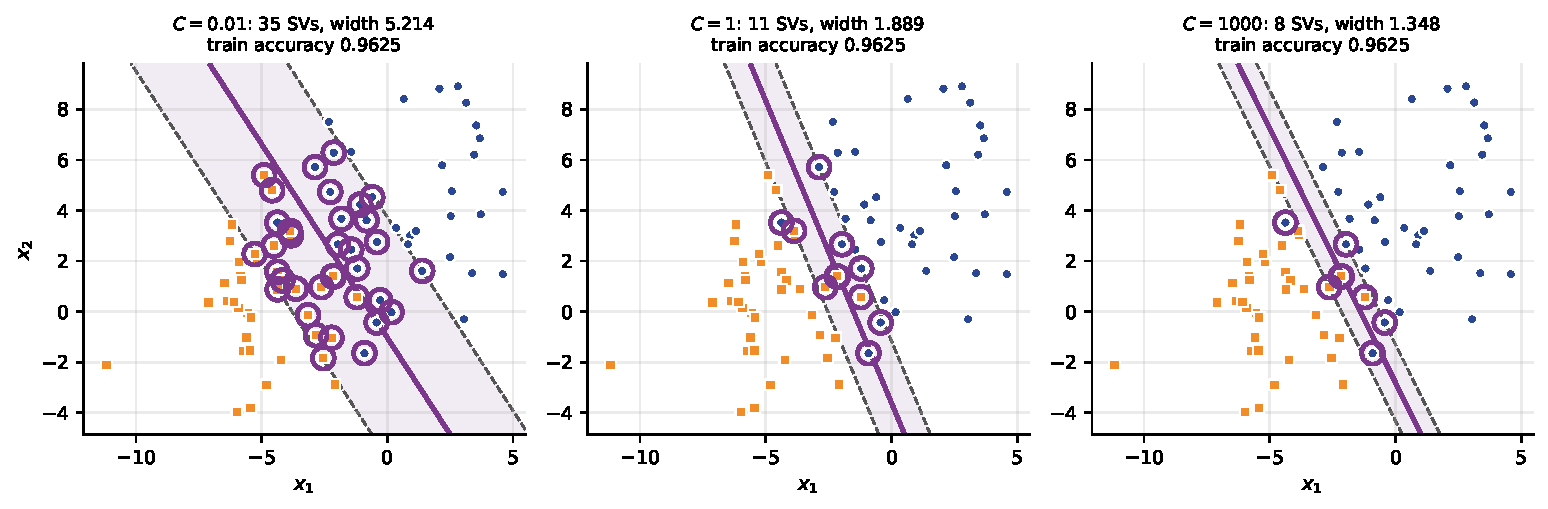
\includegraphics[width=0.88\textwidth]{softc.pdf}
  \end{center}
  \begin{center}\small
    Left to right, $C = 0.01$, $1$, $1000$. The shaded band narrows; the
    ringed support vectors go from $35$ to $8$. Small $C$ means a
    \emph{soft}, tolerant, well-populated margin.
  \end{center}
\end{frame}

\begin{frame}[fragile,shrink=5]{Strong duality, and the three kinds of $\alpha$}
\begin{outblk}
primal  (1/2)||w||^2 + C*sum(hinge) = 8.184919
dual    sum(a) - 1/2 sum a_i a_j y_i y_j x_i.x_j = 8.184597
gap                                  = 3.22e-04
0 < alpha < C  (on the margin)  : 3 points
alpha = C      (inside or wrong): 8 points
alpha = 0      (spectators)     : 69 points
\end{outblk}
  \begin{center}\small
    The gap of $3.22\times 10^{-4}$ is the solver's stopping tolerance
    (\texttt{libsvm} defaults to $10^{-3}$), not a real duality gap: for a
    convex QP the gap at the true optimum is zero. \textbf{The $11$ support
    vectors are the $3$ on the margin plus the $8$ at the ceiling.}
  \end{center}
\end{frame}

\begin{frame}{Predict first \#3 --- is a large $C$ more or less regularised?}
  \begin{alertblock}{Commit before you look}
    \texttt{breast\_cancer}, scaled, linear kernel, five-fold
    cross-validation. I sweep $C$ from $0.001$ to $100$.

    \medskip
    \centering\large
    Does $\|w\|$ go \textbf{up} or \textbf{down} as $C$ grows? And which end
    of the sweep is the \emph{more} regularised model?
  \end{alertblock}
  \onslide<2->{
  \begin{exampleblock}{}
    \centering
    $\|w\|$ climbs from $\mathbf{0.3555}$ to $\mathbf{20.8998}$.\\[0.3em]
    \textbf{Large $C$ is \emph{less} regularisation.} Most of the room gets
    this backwards.
  \end{exampleblock}}
\end{frame}

\begin{frame}[fragile,shrink=6]{$C$ is inverse regularisation --- and here is why}
\begin{outblk}
      C      ||w||    5-fold CV   nSV
  0.001     0.3555   0.9385      252
   0.01     0.7265   0.9701      118
    0.1     1.4800   0.9772      60
      1     3.0669   0.9754      40
     10     7.9741   0.9631      37
    100    20.8998   0.9613      31
large C -> large ||w|| -> narrow margin -> LESS regularisation
\end{outblk}
  \begin{columns}[T]
    \begin{column}{0.48\textwidth}
      \begin{block}{Divide the objective by $C$}
        $\tfrac12\|w\|^2 + C\sum\xi_i$
        \ \ becomes \ \
        $\frac{1}{2C}\|w\|^2 + \sum\xi_i$.
        The penalty on $\|w\|^2$ is $1/(2C)$ --- so it is
        $\lambda = 1/C$ that plays the role of ridge's $\lambda$.
      \end{block}
    \end{column}
    \begin{column}{0.48\textwidth}
      \begin{alertblock}{The mnemonic}
        \centering
        \textbf{Big $C$ = big Cost of error = the model tries hard to fit
        every point = complex model.}\\[0.3em]
        \normalsize\small Best CV here is $\mathbf{0.9772}$ at $C=0.1$, and
        both ends are worse. It is a genuine tuning parameter.
      \end{alertblock}
    \end{column}
  \end{columns}
\end{frame}

\begin{frame}{The validation curve, drawn}
  \begin{center}
    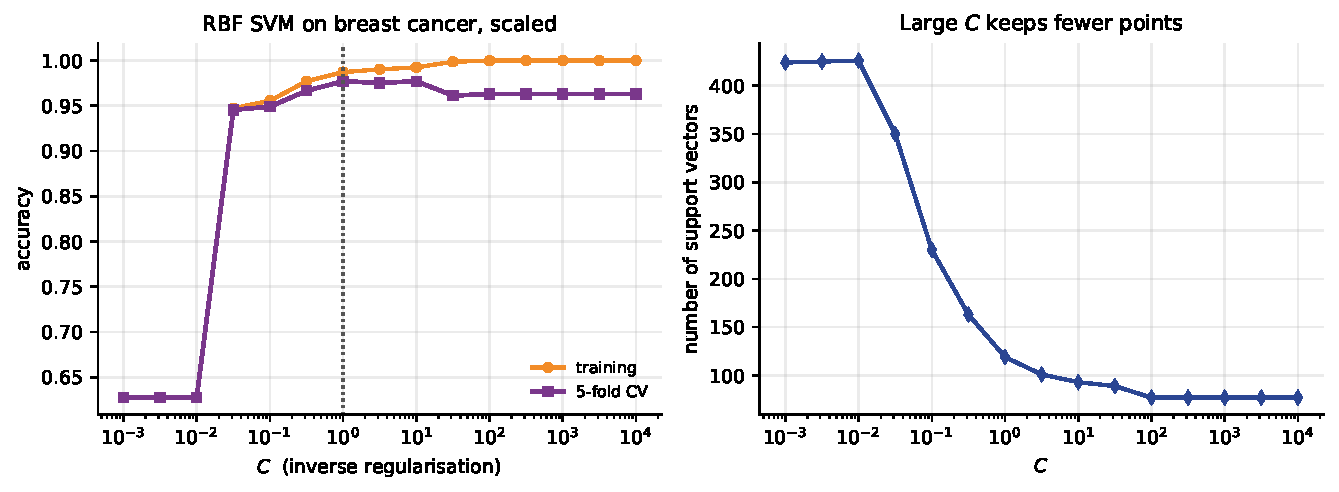
\includegraphics[width=0.72\textwidth]{cvalid.pdf}
  \end{center}
  \begin{center}\small
    Training accuracy climbs monotonically to $1.0000$ and stays there;
    cross-validated accuracy peaks at $\mathbf{0.9771}$ near $C = 1$ and
    then falls to $0.9631$. The support-vector count drops from $426$ to
    $77$ across the same sweep. \textbf{The gap between the two curves is
    the diagnostic}, not either curve alone.
  \end{center}
\end{frame}

% =====================================================================
\section[Hinge loss]{The loss the SVM minimises}
\label{sec:hinge}

\begin{frame}[shrink=14]{You have already met this function}
  \begin{block}{Eliminate the slack variables}
    At the optimum, $\xi_i$ is as small as its constraints allow:
    $\xi_i = \max(0,\,1 - y_i f(x_i))$. Substitute, and the constrained
    problem becomes an \emph{unconstrained} one:
    \[
      \min_{w,b}\ \ \underbrace{\sum_{i=1}^{n}\max\bigl(0,\ 1 - y_i f(x_i)\bigr)}
        _{\textbf{hinge loss}}
      \;+\; \frac{1}{2C}\,\|w\|^2 .
    \]
    The hinge loss came up in the loss-functions lecture as a curve on a
    graph. \textbf{The SVM is the model whose loss that is.}
  \end{block}
  \begin{center}
    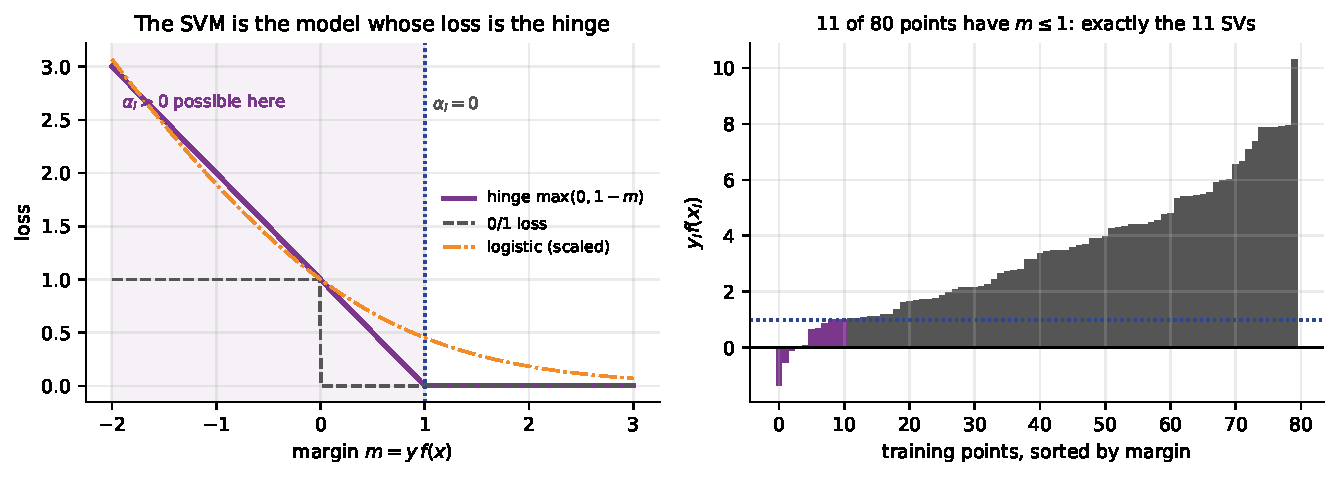
\includegraphics[width=0.80\textwidth]{hinge.pdf}
  \end{center}
  \begin{center}\small
    The hinge is \textbf{exactly zero} for $m > 1$, so a point comfortably
    outside the margin contributes no loss \emph{and no gradient}: its
    multiplier is zero and it is not a support vector. Right panel:
    $\mathbf{11}$ of $80$ points have $m \le 1$ --- and
    \texttt{n\_support\_} is $\mathbf{11}$. The same eleven.
  \end{center}
\end{frame}

\begin{frame}[fragile,shrink=8]{Same loss, two different solvers; and against logistic}
\begin{outblk}
LinearSVC(loss='hinge', C=0.01)
   ||w|| = 0.7599   mean hinge = 0.104136   objective = 0.8812   acc = 0.9842
SGDClassifier(loss='hinge', matched alpha)
   ||w|| = 0.7389   mean hinge = 0.105196   objective = 0.8716   acc = 0.9719
same loss, same regulariser, two different solvers
\end{outblk}
\begin{outblk}
SVC(linear)          uses 40 of 569 rows (the support vectors)
LogisticRegression   uses 569 of 569 rows (every one has a gradient)
cosine between the two weight vectors = 0.9132
5-fold CV  SVC 0.9754   LogisticRegression 0.9789
\end{outblk}
  \begin{center}\small
    Logistic loss is never exactly zero, so \emph{every} row contributes a
    gradient forever --- no sparsity, but smooth probabilities. The two
    weight vectors point almost the same way (cosine $0.9132$) and score
    within $0.0035$ of each other. \textbf{Different loss, similar answer,
    very different internals.}
  \end{center}
\end{frame}

% =====================================================================
\section[Kernels]{The kernel trick}
\label{sec:kernel}

\begin{frame}[shrink=4]{A problem no line can solve}
  \begin{columns}[T]
    \begin{column}{0.46\textwidth}
      \begin{block}{Concentric circles}
        $220$ points, an inner blob and an outer ring. The class is
        determined entirely by the \emph{radius}. No straight line in the
        plane can express ``inside a circle''.
      \end{block}
      \begin{alertblock}{Measured}
        A linear SVM scores $\mathbf{0.5682}$ on its own training data ---
        barely above the majority class. It is not badly tuned; the model
        class cannot do it.
      \end{alertblock}
    \end{column}
    \begin{column}{0.50\textwidth}
      \begin{exampleblock}{The idea}
        Add a column. Let
        \[ z = x_1^2 + x_2^2 . \]
        In $(x_1,x_2,z)$ space the inner blob sits low and the ring sits
        high, and a \textbf{flat plane} $z = c$ separates them.
      \end{exampleblock}
      \begin{block}{}
        \small Coming back down to two dimensions, that plane is a circle.
        Linear model, curved boundary.
      \end{block}
    \end{column}
  \end{columns}
\end{frame}

\begin{frame}[fragile,shrink=7]{Lift, separate, come back down}
  \begin{center}
    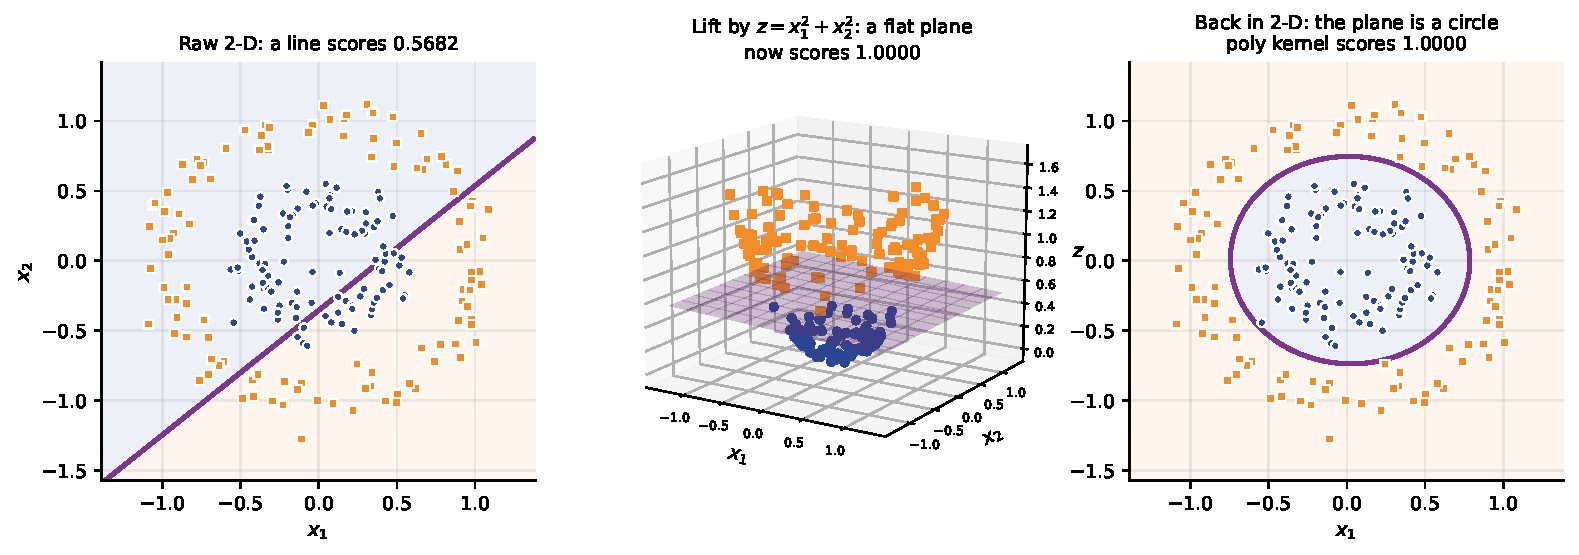
\includegraphics[width=0.94\textwidth]{kernelmap.pdf}
  \end{center}
\begin{outblk}
linear SVM, raw (x1,x2)             accuracy 0.5682
linear SVM, (x1,x2,x1^2+x2^2)       accuracy 1.0000
degree-2 polynomial kernel, raw     accuracy 1.0000
the lifted plane: w = [ 0.2076 -0.0436  6.3956]  b = -3.4436
\end{outblk}
  \begin{center}\small
    $0.5682 \to \mathbf{1.0000}$ from one extra column. And look at $w$: the
    two original coordinates get weights near zero, the radius column gets
    $6.3956$. The model found the right feature by itself.
  \end{center}
\end{frame}

\begin{frame}[shrink=6]{The trick: never build the new columns}
  \begin{block}{The map, written out}
    For $x = (x_1,x_2)$, define the degree-two feature map
    \[
      \varphi(x) = \bigl(1,\ \sqrt2\,x_1,\ \sqrt2\,x_2,\
                      x_1^2,\ x_2^2,\ \sqrt2\,x_1x_2\bigr)
      \ \in\ \mathbb{R}^6 .
    \]
  \end{block}
  \begin{columns}[T]
    \begin{column}{0.48\textwidth}
      \begin{exampleblock}{The claim}
        \[
          \langle \varphi(x), \varphi(z)\rangle
          \;=\; \bigl(1 + \langle x, z\rangle\bigr)^2 .
        \]
        Left side: build two 6-vectors, then multiply. Right side: one dot
        product in 2-D, add one, square.
      \end{exampleblock}
    \end{column}
    \begin{column}{0.48\textwidth}
      \begin{alertblock}{Why it matters}
        The dual needs $\langle x_i, x_j\rangle$ and \emph{nothing else}.
        Replace every one with $K(x_i,x_j)$ and you have trained a linear
        SVM in the six-dimensional space --- \textbf{without ever writing
        down a six-dimensional vector}.
      \end{alertblock}
    \end{column}
  \end{columns}
  \begin{center}\small
    That claim is an identity. We are going to check it, not believe it.
  \end{center}
\end{frame}

\begin{frame}[fragile,shrink=6]{Verified by hand: $x = (1,2)$, $z = (3,1)$}
\begin{outblk}
x = [1. 2.]   z = [3. 1.]
x.z            = 5.0000000000
(1 + x.z)^2    = 36.0000000000
phi(x) = [1.       1.414214 2.828427 1.       4.       2.828427]
phi(z) = [1.       4.242641 1.414214 9.       1.       4.242641]
phi(x).phi(z)  = 36.0000000000
difference     = 0.00e+00
2 features -> 6, and the kernel never built either vector
\end{outblk}
  \begin{center}\small
    Do the right-hand side with a pen: $x\cdot z = 3 + 2 = 5$, and
    $(1+5)^2 = 36$. Now the left-hand side, term by term:
    $1 + 6 + 4 + 9 + 4 + 12 = 36$. \textbf{The same number, and the
    difference is exactly zero.}
  \end{center}
\end{frame}

\begin{frame}[fragile,shrink=6]{And over a whole dataset, not one lucky pair}
\begin{lstlisting}
V = rng.normal(size=(200, 2))
Kk  = (1 + V @ V.T) ** 2                     # the kernel, 2-D arithmetic
Phi = np.array([phi2(v) for v in V])         # the explicit 6-D map
Ke  = Phi @ Phi.T                            # its Gram matrix
\end{lstlisting}
\begin{outblk}
kernel matrix       : 200 x 200
explicit map        : 200 x 6, then a 200 x 200 Gram matrix
max |K - phi phi^T| = 2.842e-14
max |K - sklearn|   = 0.000e+00
multiplications, explicit map: 240000
multiplications, kernel      : 80000
\end{outblk}
  \begin{center}\small
    $40\,000$ entries and the worst disagreement is
    $2.8\times10^{-14}$ --- floating point, not mathematics. Against
    \texttt{polynomial\_kernel} it is $\mathbf{0}$.
  \end{center}
\end{frame}

\begin{frame}[fragile,shrink=6]{The map you did not have to build}
\begin{outblk}
d =   2, degree 2 -> explicit map has        6 features
d =  10, degree 2 -> explicit map has       66 features
d =  10, degree 3 -> explicit map has      286 features
d =  30, degree 3 -> explicit map has     5456 features
d =  30, degree 5 -> explicit map has   324632 features
d = 100, degree 3 -> explicit map has   176851 features
d = 100, degree 5 -> explicit map has 96560646 features
the kernel evaluates every one of them with d + 1 multiplications
\end{outblk}
  \begin{center}\small
    The count is $\binom{d+p}{p}$. At $d = 100$ and degree $5$ the explicit
    map has \textbf{ninety-six million} columns, and
    $(1 + x^\top z)^5$ costs a hundred multiplications, one addition and one
    power. This is not an optimisation --- it is the difference between
    possible and impossible.
  \end{center}
\end{frame}

\begin{frame}[fragile,shrink=6]{The kernel machine \emph{is} the explicit-map machine}
\begin{lstlisting}
Pk = SVC(kernel="poly", degree=2, gamma=1.0, coef0=1.0, C=1.0).fit(Xr, yr)
Pe = SVC(kernel="linear", C=1.0).fit(np.array([phi2(v) for v in Xr]), yr)
\end{lstlisting}
\begin{outblk}
kernel machine, first five f(x) : [-1.110765  1.463534  2.436074 -1.060217 -1.397726]
explicit map,   first five f(x) : [-1.110765  1.463534  2.436074 -1.060217 -1.397726]
max |difference|                = 1.24e-14
identical predictions           : True
support vectors: kernel 38, explicit 38
\end{outblk}
  \begin{center}\small
    Not merely the same predictions --- the same \emph{decision function
    values}, to fourteen decimal places, and the same $38$ support vectors.
    They are one model, computed two ways.
  \end{center}
\end{frame}

\begin{frame}[fragile,shrink=6]{The RBF kernel, where there is no map to build}
  \[
    K(x,z) = \exp\bigl(-\gamma\,\|x - z\|^2\bigr)
  \]
\begin{outblk}
gamma =   0.1   exp(-g||u-v||^2) = 0.8994246481   sklearn = 0.8994246481
gamma =     1   exp(-g||u-v||^2) = 0.3464558103   sklearn = 0.3464558103
gamma =    10   exp(-g||u-v||^2) = 0.0000249160   sklearn = 0.0000249160
||u-v||^2 = 1.0600
\end{outblk}
  \begin{columns}[T]
    \begin{column}{0.48\textwidth}
      \begin{block}{Expand the exponential}
        $e^{t}$ has infinitely many terms, so the implied feature map has
        infinitely many coordinates. You could never write it down.
      \end{block}
    \end{column}
    \begin{column}{0.48\textwidth}
      \begin{alertblock}{And you never need to}
        The kernel is one subtraction, one norm and one \texttt{exp}. An
        SVM can therefore fit a linear model in an
        infinite-dimensional space using arithmetic that fits on this slide.
      \end{alertblock}
    \end{column}
  \end{columns}
\end{frame}

\begin{frame}[fragile,shrink=6]{Three kernels on the same two moons}
\begin{outblk}
kernel        nSV   train    5-fold CV
linear         86   0.8667   0.8583
poly deg 2     84   0.8542   0.8417
poly deg 3     53   0.9458   0.9417
rbf g=1        64   0.9583   0.9458
\end{outblk}
  \begin{center}
    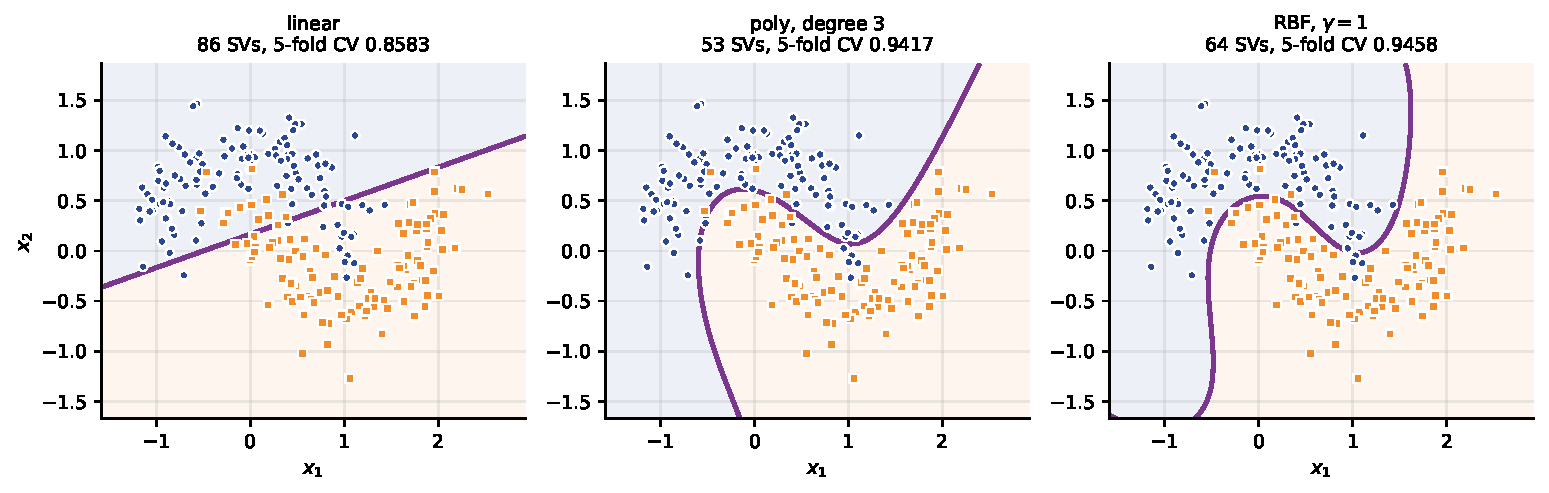
\includegraphics[width=0.80\textwidth]{kernels.pdf}
  \end{center}
  \begin{center}\small
    Degree \emph{two} is worse than linear here ($0.8417$ against $0.8583$).
    An even-degree polynomial is symmetric in a way this data is not. More
    flexibility is not automatically better --- it has to be the
    \emph{right} flexibility.
  \end{center}
\end{frame}

% =====================================================================
\section[Practice]{$\gamma$, scaling and what it all costs}
\label{sec:practice}

\begin{frame}[fragile,shrink=7]{$\gamma$ is how far one training point reaches}
\begin{outblk}
 gamma   distance at which K falls to 0.01   nSV   train   5-fold CV
  0.01             21.4597              158   0.8208   0.8167
   0.1              6.7861              103   0.8542   0.8542
     1              2.1460               64   0.9583   0.9458
    10              0.6786               89   0.9708   0.9625
   100              0.2146              212   0.9917   0.9125
\end{outblk}
  \begin{center}
    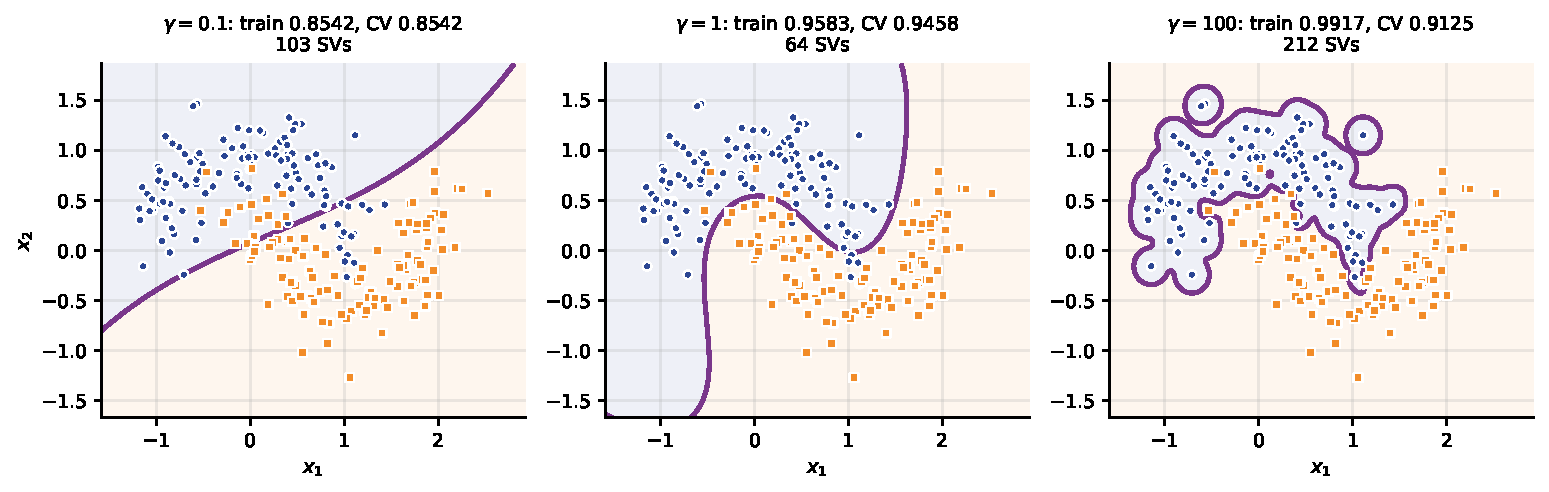
\includegraphics[width=0.80\textwidth]{gammaboundary.pdf}
  \end{center}
  \begin{center}\small
    Small $\gamma$: every point influences the whole plane, and the boundary
    is nearly straight. Large $\gamma$: influence dies within $0.21$ units,
    so the model builds an island around each training point.
  \end{center}
\end{frame}

\begin{frame}[fragile,shrink=6]{Large $\gamma$ overfits, and it is spectacular}
\begin{outblk}
  gamma    train    5-fold CV    nSV of 569
  0.001    0.9525    0.9455       200
   0.01    0.9824    0.9701       111
    0.1    0.9912    0.9596       221
      1    1.0000    0.6309       568
     10    1.0000    0.6274       569
majority class = 0.6274
\end{outblk}
  \begin{center}
    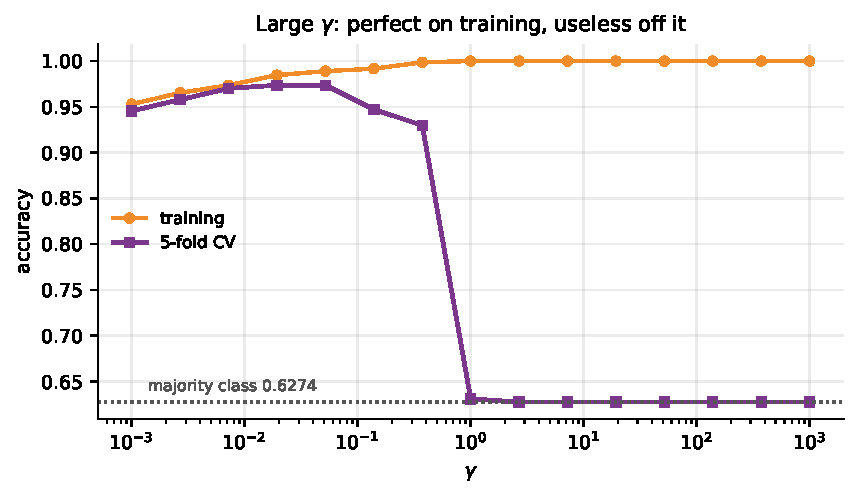
\includegraphics[width=0.62\textwidth]{gammacurve.pdf}
  \end{center}
  \begin{center}\small
    At $\gamma = 10$: training $\mathbf{1.0000}$, cross-validated
    $\mathbf{0.6274}$ --- \emph{exactly} the majority-class rate, and
    \textbf{569 of 569} rows are support vectors. The model has memorised
    every row and generalises to nothing.
  \end{center}
\end{frame}

\begin{frame}{Predict first \#4 --- what happens if you skip the scaler?}
  \begin{alertblock}{Commit to a number}
    \texttt{breast\_cancer} has $30$ columns. The widest has standard
    deviation $568.86$; the narrowest, $0.002644$. That is a ratio of
    $\mathbf{215\,171}$.

    \medskip
    \centering\large
    How much cross-validated accuracy does an RBF SVM lose if you fit the raw
    columns instead of standardising them first?
  \end{alertblock}
  \onslide<2->{
  \begin{exampleblock}{}
    \centering\large
    $0.9210$ raw against $\mathbf{0.9771}$ scaled --- a loss of
    $\mathbf{0.0561}$.
  \end{exampleblock}
  \begin{center}\small
    Fifty-six patients in a thousand, given away by one missing line of code.
  \end{center}}
\end{frame}

\begin{frame}[fragile,shrink=6]{Scaling is not optional --- with one honest exception}
\begin{outblk}
breast_cancer: widest column sd 568.8565, narrowest 0.002644, ratio 215170.7
model                           raw   scaled      gap
SVC(rbf, gamma='scale')      0.9210   0.9771  +0.0561
SVC(rbf, gamma=1)            0.6274   0.6309  +0.0035
SVC(linear)                  0.9526   0.9754  +0.0229
SVC(poly, degree 3)          0.9122   0.8981  -0.0142
\end{outblk}
  \begin{columns}[T]
    \begin{column}{0.50\textwidth}
      \begin{block}{Why it bites so hard}
        $\|x - z\|^2$ is dominated by whichever column has the largest
        numbers. One column with an $s.d.$ of $569$ drowns out
        twenty-nine others, so the RBF kernel effectively sees a
        one-feature problem.
      \end{block}
    \end{column}
    \begin{column}{0.46\textwidth}
      \begin{alertblock}{Report the row that disagrees}
        The degree-3 polynomial got \textbf{worse} when scaled,
        $-0.0142$. It happens; do not hide it. Scaling is a reliable default,
        not a theorem --- and both of its poly scores are below the scaled
        RBF anyway.
      \end{alertblock}
    \end{column}
  \end{columns}
  \begin{center}\small
    Always inside a \texttt{Pipeline}, never as a separate step on the whole
    table: fitting the scaler on the test rows is leakage.
  \end{center}
\end{frame}

\begin{frame}[fragile,shrink=5]{The whole recipe, in six lines}
\begin{lstlisting}
pipe = Pipeline([("scale", StandardScaler()), ("svm", SVC(kernel="rbf"))])
grid = {"svm__C": [0.1, 1, 10, 100], "svm__gamma": [0.001, 0.01, 0.1, 1]}
gs = GridSearchCV(pipe, grid, cv=StratifiedKFold(5, shuffle=True,
                  random_state=0)).fit(Xtr, ytr)
\end{lstlisting}
\begin{outblk}
best parameters : {'svm__C': 100, 'svm__gamma': 0.001}
best CV score   : 0.9859
held-out score  : 0.9580
support vectors : 43 of 426 training rows
\end{outblk}
  \begin{center}\small
    Note the held-out score is \emph{below} the cross-validated one:
    $0.9580$ against $0.9859$. That gap is the optimism of having chosen
    the best of sixteen configurations. \textbf{Report the held-out number.}
    And note $C$ and $\gamma$ traded off --- a large $C$ with a tiny
    $\gamma$.
  \end{center}
\end{frame}

\begin{frame}[fragile,shrink=9]{What it costs as the data grows --- count first}
\begin{outblk}
     n     nSV easy   nSV hard   kernel entries n^2
   500        248        380               250000
  2000        624       1097              4000000
  8000       1604       3108             64000000
 32000       4596       9280           1024000000
nSV grows as n^0.69 (class_sep 0.9) and n^0.76 (class_sep 0.4)
64x the rows gives 18.5x the support vectors on the easy problem and
24.4x on the hard one; the kernel matrix grows 4096x either way
\end{outblk}
  \begin{center}\small
    \textbf{These are exact}, and the same on your machine as on mine. The
    kernel matrix grows as $n^2$; the support-vector set grows as
    $n^{0.69}$. The cost lives between the two, which is why the measured
    exponent lands between $1$ and $2$.
  \end{center}
\end{frame}

\begin{frame}[fragile,shrink=9]{And now the clock, with a health warning}
\begin{outblk}
     n   SVC(rbf) fit   nSV / n   LinearSVC fit    ratio
   500         0.003 s     0.50          0.001 s      3.6x
  2000         0.024 s     0.31          0.002 s     13.6x
  8000         0.257 s     0.20          0.005 s     47.1x
 32000         3.308 s     0.14          0.048 s     68.7x
MACHINE-DEPENDENT: time ~ n^1.72 (easy), n^1.81 (hard), n^0.98 (LinearSVC)
\end{outblk}
  \begin{center}
    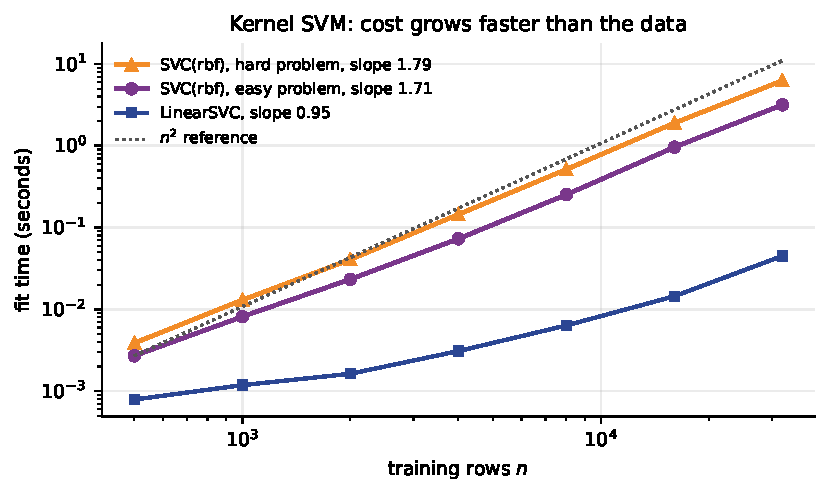
\includegraphics[width=0.46\textwidth]{cost.pdf}
  \end{center}
  \begin{center}\small
    \textbf{A seed cannot fix a clock.} Repeated runs on this machine moved
    the exponent between $n^{1.68}$ and $n^{1.72}$. Quote the counts.
  \end{center}
\end{frame}

\begin{frame}[shrink=6]{Be precise about the exponent}
  \begin{columns}[T]
    \begin{column}{0.50\textwidth}
      \begin{alertblock}{What the textbook says}
        Kernel SVM training is between $O(n^2)$ and $O(n^3)$, because the
        kernel matrix alone has $n^2$ entries.
      \end{alertblock}
      \begin{block}{What we measured}
        An exponent \emph{below} quadratic on both problems --- so say so,
        and then explain it.
      \end{block}
    \end{column}
    \begin{column}{0.46\textwidth}
      \begin{exampleblock}{And the reason is in the table}
        The support-vector fraction \textbf{falls} as $n$ grows:
        $0.50 \to 0.14$. \texttt{libsvm} caches and shrinks, and the work is
        driven by the support vectors, not the rows. Make the problem harder
        --- keep more support vectors --- and the \emph{count} exponent
        climbs from $0.69$ to $0.76$, and the time follows it.
      \end{exampleblock}
    \end{column}
  \end{columns}
  \begin{center}\small
    The practical conclusion survives intact, stated in counts: $64\times$
    the rows gives $\mathbf{18.5\times}$ the support vectors and
    $\mathbf{4096\times}$ the kernel matrix. Beyond roughly $10^5$ rows, use
    \texttt{LinearSVC} --- which never forms that matrix --- or
    \texttt{SGDClassifier}.
  \end{center}
\end{frame}

\begin{frame}[fragile,shrink=13]{Prediction is not free either --- and there are only two sides}
\begin{outblk}
C =   0.01  nSV =  5988  kernel evaluations to score 8000 rows = 47904000
C =      1  nSV =  1604  kernel evaluations to score 8000 rows = 12832000
C =    100  nSV =  1368  kernel evaluations to score 8000 rows = 10944000
\end{outblk}
  \begin{columns}[T]
    \begin{column}{0.50\textwidth}
      \begin{block}{Why}
        \[
          f(x) = \sum_{i \in \mathrm{SV}} \alpha_i y_i K(x_i, x) + b .
        \]
        Every prediction is a sum over the support vectors, so scoring
        $8000$ rows costs exactly $8000 n_{\mathrm{SV}}$ kernel evaluations
        --- $4.4\times$ more at $C = 0.01$ than at $C = 100$, on any machine. An RBF SVM
        is a \emph{learned}, weighted, sparse nearest-neighbour rule --- and
        it inherits k-NN's prediction-time cost.
      \end{block}
    \end{column}
    \begin{column}{0.48\textwidth}
\begin{outblk}
classes            : 3
pairwise SVMs      : 3  (= k(k-1)/2)
dual_coef_ shape   : (2, 51)
n_support_ per class: [ 8 22 21]
decision_function  : (1, 3) one per pair
5-fold CV accuracy : 0.9533
\end{outblk}
      \begin{center}\small
        An SVM is intrinsically a \textbf{two-class} machine: one hyperplane,
        two sides. \texttt{SVC} handles $k$ classes with $k(k-1)/2$
        one-against-one machines and a vote. At $k=10$ that is $45$ models.
      \end{center}
    \end{column}
  \end{columns}
\end{frame}

% =====================================================================
\section{Summary}
\label{sec:summary}

\begin{frame}[shrink=24]{Summary --- twelve lines}
  \begin{enumerate}\small
    \item Many hyperplanes separate a separable set and accuracy cannot rank
      them. Of five perfect lines on the six points, clearance ranged from
      $0.0707$ to $\mathbf{0.7071}$.
    \item The signed distance to $w^\top x + b = 0$ is $(w^\top x+b)/\|w\|$.
      Fix the scale so the closest points have $y_i f(x_i) = 1$, and the band
      has width $\mathbf{2/\|w\|}$. Maximising it is minimising
      $\tfrac12\|w\|^2$ --- a convex QP with one global optimum.
    \item The Lagrangian gives $w = \sum_i \alpha_i y_i x_i$ and
      $\sum_i \alpha_i y_i = 0$; substituting yields the dual, in which the
      data appears \textbf{only} as $\langle x_i, x_j\rangle$.
    \item Complementary slackness
      $\alpha_i[y_i f(x_i) - 1] = 0$ forces every point to have either
      $\alpha_i = 0$ or $y_i f(x_i) = 1$. The rest are
      \textbf{support vectors}.
    \item Six points by hand: $\alpha_A = \alpha_D = 1$, $w = (1,1)$,
      $b = -3$, width $\mathbf{1.414214}$. \texttt{SVC(kernel='linear',
      C=1e6)} returns the identical numbers to $10^{-9}$.
    \item Deleting non-support-vector B moved $w$ by
      $\mathbf{0.00\mathrm{e}{+}00}$. Deleting support vector A moved
      $w$ to $(0.6664, 0.6668)$ and widened the margin to $2.1215$.
      Refitting on the $11$ support vectors of an $80$-point problem gave
      identical predictions on all $80$.
    \item Soft margin: $\xi_i \ge 0$, objective
      $\tfrac12\|w\|^2 + C\sum\xi_i$, dual unchanged except
      $0 \le \alpha_i \le C$. Across $C = 0.01 \to 1000$ the width went
      $5.2135 \to 1.3483$ and points inside the margin $32 \to 5$, while
      training accuracy stayed at $0.9625$ throughout.
    \item $C$ is \textbf{inverse} regularisation: $\|w\|$ climbed
      $0.3555 \to 20.8998$ as $C$ went $0.001 \to 100$, and CV peaked at
      $\mathbf{0.9772}$ in the middle.
    \item Eliminating $\xi$ gives
      $\sum \max(0, 1 - y_i f(x_i)) + \frac{1}{2C}\|w\|^2$: the SVM is the
      model whose loss is the \textbf{hinge}. It is flat beyond $m=1$, which
      is exactly why most $\alpha_i$ are zero --- $11$ of $80$ points had
      $m \le 1$ and \texttt{n\_support\_} was $11$.
    \item Kernels: $\langle\varphi(x),\varphi(z)\rangle = (1+x^\top z)^2$
      \textbf{verified} to $0.00\mathrm{e}{+}00$ at $x=(1,2)$, $z=(3,1)$
      (both sides $36$), and to $2.8\times10^{-14}$ over a $200\times200$
      Gram matrix. Kernel machine and explicit-map machine agree to
      $1.24\times10^{-14}$ with the same $38$ support vectors. Circles:
      $0.5682 \to \mathbf{1.0000}$.
    \item $\gamma$ is a reach. On \texttt{breast\_cancer},
      $\gamma = 10$ gives train $1.0000$, CV $\mathbf{0.6274}$ (the
      majority-class rate) and $569/569$ support vectors. Without
      \texttt{StandardScaler} the RBF SVM loses $\mathbf{0.0561}$ --- the
      column standard deviations differ by a factor of $215\,171$.
    \item Cost: $64\times$ the rows gives $18.5\times$ the support vectors
      and $4096\times$ the kernel matrix --- exact. The measured time
      exponent lands below the documented $O(n^2)$--$O(n^3)$ for that reason.
      Prediction cost scales with the number of support vectors.
      Past $\sim10^5$ rows, use \texttt{LinearSVC}.
  \end{enumerate}
\end{frame}

\begin{frame}[shrink=4]{Before the next lecture}
  \begin{columns}[T]
    \begin{column}{0.48\textwidth}
      \begin{block}{Read}
        \texttt{notes.pdf} --- the $2/\|w\|$ derivation in full, the
        Lagrangian and the dual step by step, the six points solved twice,
        and \textbf{ten practice questions with full worked solutions}.
      \end{block}
      \begin{block}{Do}
        Reproduce the six-point solution with a pen: guess the support set,
        use $\sum\alpha_i y_i = 0$ and the two margin equations, get
        $\alpha = 1$, $w = (1,1)$, $b = -3$. Then verify
        $(1 + x^\top z)^2 = \langle\varphi(x),\varphi(z)\rangle$ for
        $x = (1,2)$, $z = (3,1)$ by expanding both sides.
      \end{block}
    \end{column}
    \begin{column}{0.48\textwidth}
      \begin{exampleblock}{The habit to take away}
        \texttt{make\_pipeline(StandardScaler(), SVC())} and a grid over
        $C$ and $\gamma$. Never an \texttt{SVC} on raw columns; never $C$ or
        $\gamma$ chosen on the training score.
      \end{exampleblock}
      \begin{alertblock}{And the habit to unlearn}
        ``Large $C$ regularises more.'' It is the opposite:
        $\lambda = 1/C$. If you remember one sentence from the soft-margin
        section, make it that one.
      \end{alertblock}
    \end{column}
  \end{columns}
  \begin{center}
    \small Materials: \texttt{\AMLRepoURL}
  \end{center}
  \slidesources{\AMLUnitVISources}
\end{frame}

\end{document}
